\section{Implementation}
\label{sec:implementation}

\subsection{Modulation}
\subsubsection{Triangle Wave Generator}
The topology implemented for this subcircuit was found in \citetitle{TriangleWaveTopology}\cite{TriangleWaveTopology}. 
It uses an integrator to generate a ramp from the output of a non-inverting schmitt trigger. 
This ramp is fed into the input of the schmitt trigger. When the ramp reaches a schmitt trigger threshold, the polarity of the schmitt trigger output reverses, forcing the integrator to ramp in the opposite direction. 
High precision, rail-to-rail opamps and E96 resistors ensure the amplitude and offset tolerances were met. 

Figure \ref{fig:triangleWaveGeneratorSchematic} shows the schematic, and Figure \ref{fig:triangleWaveGeneratorTestBench} shows the testbench used to test it. 
The Spice error log shows the results of the measurement directives.
The offset is 0.003V and the peak-to-peak voltage is 2.001 V.
The steady-state frequency is measured as 11.3532 Hz.
Each of these falls within the tolerances presented in Section \ref{sec:specificationTriangleWaveGenerator}.
A cutting of the waveform produced can be found in Figure \ref{fig:triangleWaveGeneratorWaveform}. 


\begin{figure}[H]
    \centering 
    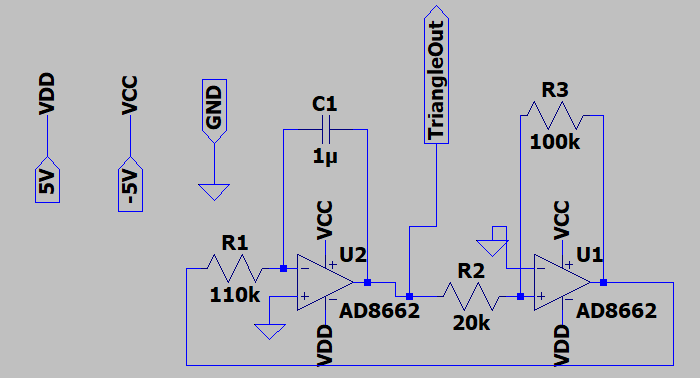
\includegraphics[width=\textwidth]{../Circuits/Images/TriangleWaveGenerator/schematic}
    \caption{A screencap of the Triangle Wave Generator Subcircuit}
    \label{fig:triangleWaveGeneratorSchematic}
\end{figure}

\begin{figure}[H]
    \centering 
    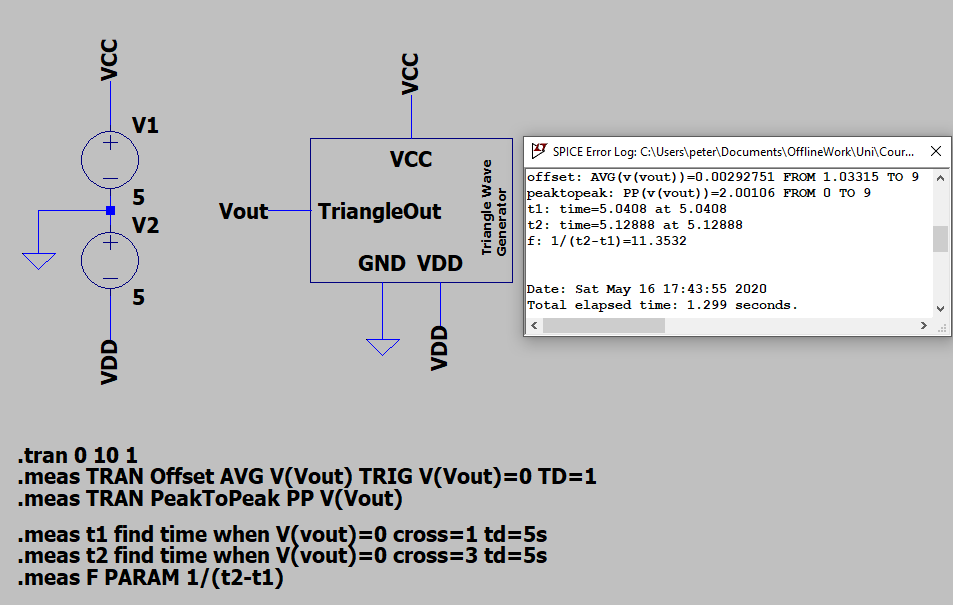
\includegraphics[width=\textwidth]{../Circuits/Images/TriangleWaveGenerator/TestBenchScreencap}
    \caption{A screencap of the Triangle Wave Generator Subcircuit}
    \label{fig:triangleWaveGeneratorTestBench}
\end{figure}

\begin{figure}[H]
    \centering 
    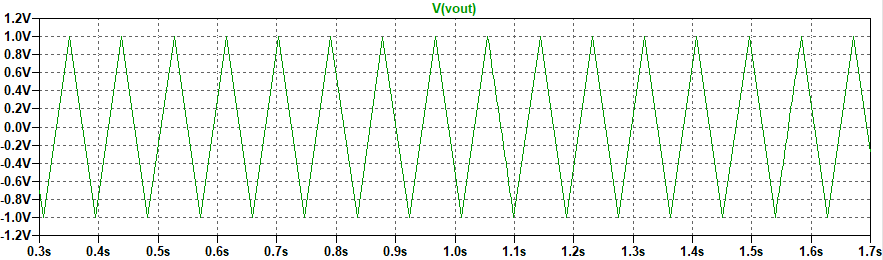
\includegraphics[width=\textwidth]{../Circuits/Images/TriangleWaveGenerator/OutputWaveform}
    \caption{A screencap of the Triangle Wave Generator Subcircuit}
    \label{fig:triangleWaveGeneratorWaveform}
\end{figure}

\subsubsection{VCO}
The VCO subcircuit is based on the LTC6990 VCO IC. 
$K_{VCO}$ and the centre frequency are set using E96 resistors.
The LTSpice schematic was adapted from a circuit generatd automatically on an online design tool provided by Analog Devices\footnote{\url{http://beta-tools.analog.com/timerblox/LTC6990}}.
The schematic is shown in Figure \ref{fig:VCOSchematic}.

The testbench varies the control voltage VC and takes frequency measurements at the appropriate times. 
The testbench is shown in Figure \ref{fig:VCOTestBench}.
The waveform produced is shown in Figure \ref{fig:VCOTestBenchWaveform}.

The measurements showed that the centre` frequency ($F_{Centre}$) is 39842 Hz and the Bandwidth of the FM Modulated signal is 7905.5 Hz.
This falls within the tolerances presented in Section \ref{sec:specificationVCO}.

This IC shifts the phase of the signal by $\pi$ radians, the FM signal frequency increases when VC drops and vica versa. 
The VCO will need to account for this. 

\begin{figure}[H]
    \centering 
    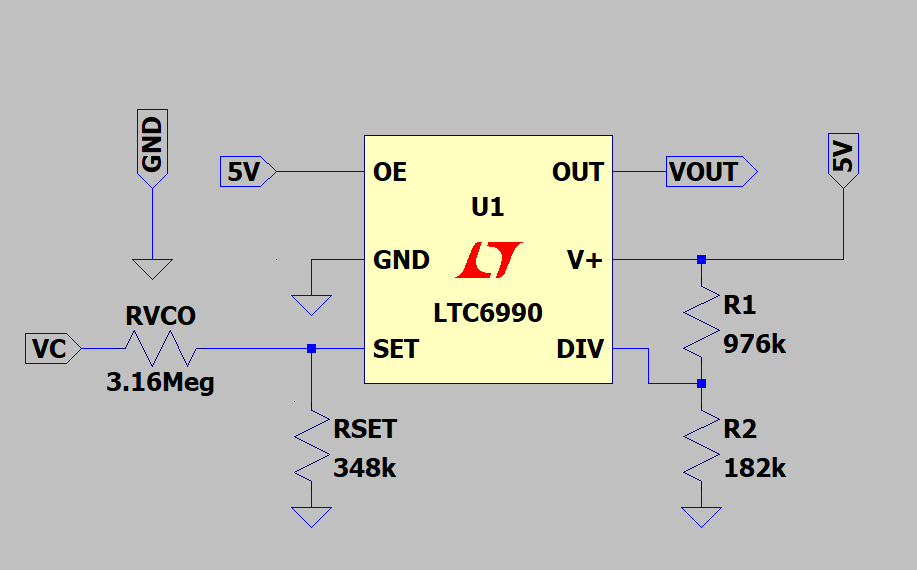
\includegraphics[width=\textwidth]{../Circuits/Images/VCO/Schematic}
    \caption{A screencap of the VCO Subcircuit}
    \label{fig:VCOSchematic}
\end{figure}

\begin{figure}[H]
    \centering 
    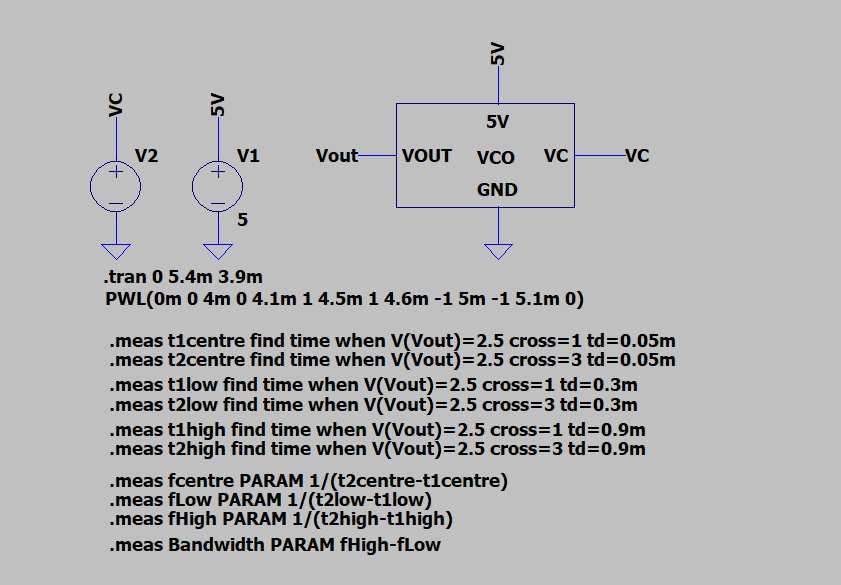
\includegraphics[width=\textwidth]{../Circuits/Images/VCO/TestBenchScreencap}
    \caption{The testbench fort the VCO Subcircuit}
    \label{fig:VCOTestBench}
\end{figure}

\begin{figure}[H]
    \centering 
    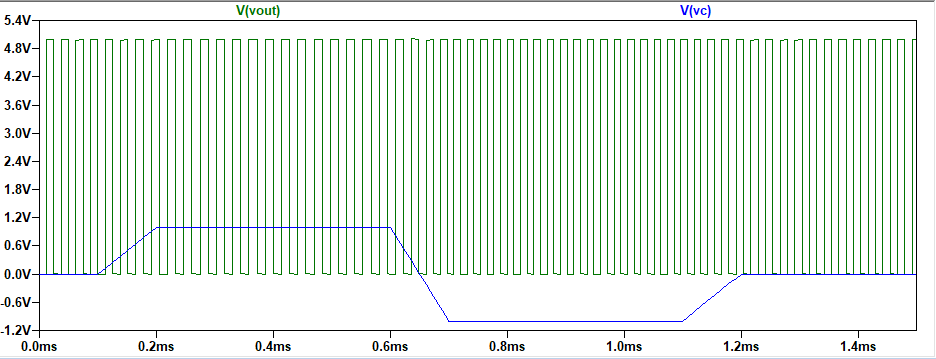
\includegraphics[width=\textwidth]{../Circuits/Images/VCO/TestBenchWaveform}
    \caption{The Waveform produced by the VCO Testbench}
    \label{fig:VCOTestBenchWaveform}
\end{figure}
